\documentclass[landscape]{article}
\usepackage[latin1]{inputenc}
\usepackage{ragged2e}
\AtBeginDocument{\RaggedRight}
\usepackage{rotating}
\usepackage{latexsym}
\usepackage{graphicx}
\usepackage{amssymb}
\renewcommand{\labelitemi}{\color{MPIIblue} $\blacktriangleright$}
\usepackage{amsmath}
\usepackage{url}
\usepackage{calc}
\usepackage[
    paperheight=20cm,
    paperwidth=40cm,
    %a4paper,
    left=4mm,
    right=4mm,
    top=2mm,
    bottom=2mm,
    includehead,
    headheight=15.5mm,
    %showframe
]{geometry}
\usepackage{fancyhdr}
\usepackage{parskip}
\usepackage{tikz}
\usepackage{tikz-3dplot}
\usepackage{pgfplots}
\usetikzlibrary{calc}
\usetikzlibrary{shadings,shadows}
\usepackage{xcolor}
\usepackage{tcolorbox}
\tcbuselibrary{skins,breakable}
\usepackage[backend=bibtex,style=numeric]{biblatex}

\pagestyle{fancy}
\makeatletter
\def\headrule{}
\def\footrule{}
\makeatother
\lfoot{}
\cfoot{}
\rfoot{}
\lhead{ %
	\hspace*{0.5mm}
	\raisebox{0mm}{
\includegraphics[height=20mm]{gfx/mpilogo-inf-narrow}}
}
\chead{%
    \vspace*{4mm}
   	\begin{center}
        {\Huge\bf Disentangling Adversarial Robustness and Generalization}\\[1.5mm]
        {\huge David Stutz, Matthias Hein and Bernt Schiele}
    \end{center}
    %\vspace*{5mm}
}
\rhead{ %
	\raisebox{2.5mm}{
\includegraphics[height=17mm]{gfx/UT_WBMW_Rot_RGB}}\hskip 2.5mm
}

\bibliography{bibliography}

\renewcommand{\rmdefault}{phv}
\renewcommand{\sfdefault}{phv}
\renewcommand{\ttdefault}{pcr}

\definecolor{MPIIblue}{RGB}{0,51,93}
\definecolor{MPIIlightblue}{RGB}{103,133,158} % 67859E
\definecolor{MPIIorange}{RGB}{200,91,15} % C85B0F
\definecolor{MPIIblack}{RGB}{46,46,46}
\definecolor{MPIIwhite}{RGB}{255,255,255}
\definecolor{MPIIdarkgray}{RGB}{123,123,123}
\definecolor{MPIIdarkergray}{RGB}{89,89,89}
\definecolor{MPIIgray}{RGB}{169,169,169}
\definecolor{MPIIlightgray}{RGB}{214,214,214}
\definecolor{MPIIlightergray}{RGB}{234,234,234}
\definecolor{MPIIgreen}{HTML}{327a2b} % 0.22,0.54, 0.19
\definecolor{MPIIred}{rgb}{0.65,0.23,0.25}
\definecolor{MPIIbeige}{rgb}{0.65,0.23,0.25}
\definecolor{MPIIpink}{HTML}{d36582}
\definecolor{MPIIteal}{HTML}{4d7c8a}
\definecolor{MPIIviolet}{HTML}{3c1642}
\definecolor{MPIIbrown}{HTML}{5a352a}
\definecolor{MPIIyellow}{HTML}{eee82c}
% pink f76f8e d36582
% teal 7180b9 4d7c8a 55dde0
% violet 3423a6 7353ba 3c1642
% light green c5d86d
% brown 230007 
% citrine d7cf07
% yellow eee82c
% brown 5a352a 60463b 423629

\newenvironment{problem}[1]{%
    \tcolorbox[noparskip,frame hidden,boxrule=0.5mm,colframe=MPIIblue,
    colbacktitle=MPIIblue,coltitle=MPIIwhite,
    colback=MPIIwhite,
    titlerule=0mm,sharpish corners,no shadow,
    left=1.5mm,top=1.5mm,right=1.5mm,bottom=1mm,
    lefttitle=1.5mm,toptitle=2mm,righttitle=1.5mm,bottomtitle=2mm,
    title=#1]}%
{\endtcolorbox}
\newenvironment{related}[1]{%
    \tcolorbox[noparskip,frame hidden,boxrule=0.5mm,colframe=MPIIgray,
    colbacktitle=MPIIgray,coltitle=MPIIwhite,
    colback=MPIIwhite,
    titlerule=0mm,sharpish corners,no shadow,
    left=1.5mm,top=1.5mm,right=1.5mm,bottom=1mm,
    lefttitle=1.5mm,toptitle=2mm,righttitle=1.5mm,bottomtitle=2mm,
    title=#1]}%
{\endtcolorbox}
\newenvironment{method}[1]{%
    \tcolorbox[noparskip,frame hidden,boxrule=0.5mm,colframe=MPIIorange,
    colbacktitle=MPIIorange,coltitle=MPIIwhite,
    colback=MPIIwhite,
    titlerule=0mm,sharpish corners,no shadow,
    left=1.5mm,top=1.5mm,right=1.5mm,bottom=1mm,
    lefttitle=1.5mm,toptitle=2mm,righttitle=1.5mm,bottomtitle=2mm,
    title=#1]}%
{\endtcolorbox}
\newenvironment{data}[1]{%
    \tcolorbox[noparskip,frame hidden,boxrule=0.5mm,colframe=MPIIgray,
    colbacktitle=MPIIgray,coltitle=MPIIwhite,
    colback=MPIIwhite,
    titlerule=0mm,sharpish corners,no shadow,
    left=1.5mm,top=1.5mm,right=1.5mm,bottom=1mm,
    lefttitle=1.5mm,toptitle=2mm,righttitle=1.5mm,bottomtitle=2mm,
    title=#1]}%
{\endtcolorbox}
\newenvironment{results}[1]{%
    \tcolorbox[noparskip,frame hidden,boxrule=0.5mm,colframe=MPIIlightgray,
    colbacktitle=MPIIlightgray,coltitle=MPIIblue,
    colback=MPIIwhite,
    titlerule=0mm,sharpish corners,no shadow,
    left=1.5mm,top=1.5mm,right=1.5mm,bottom=1mm,
    lefttitle=1.5mm,toptitle=2mm,righttitle=1.5mm,bottomtitle=2mm,
    title=#1]}%
{\endtcolorbox}
\newenvironment{moreresults}[1]{%
	\tcolorbox[noparskip,frame hidden,boxrule=0.5mm,colframe=MPIIlightgray,
	colbacktitle=MPIIwhite,coltitle=MPIIblue,
	colback=MPIIwhite,
	titlerule=0mm,sharpish corners,no shadow,
	left=1.5mm,top=1.5mm,right=1.5mm,bottom=1mm,
	lefttitle=1.5mm,toptitle=2mm,righttitle=1.5mm,bottomtitle=2mm,
	title=#1]}%
{\endtcolorbox}
\newenvironment{code}[1]{%
    \tcolorbox[noparskip,frame hidden,boxrule=0mm,colframe=MPIIwhite,
    colback=MPIIorange,coltext=MPIIwhite,
    titlerule=0mm,sharpish corners,no shadow,
    left=2.5mm,top=2.5mm,right=2.5mm,bottom=2.5mm,
    lefttitle=1.5mm,toptitle=2mm,righttitle=1.5mm,bottomtitle=2mm,
    title=#1]}%
{\endtcolorbox}
\newenvironment{references}[1]{%
    \tcolorbox[noparskip,frame hidden,boxrule=0.5mm,colframe=MPIIlightgray,
    colbacktitle=MPIIwhite,coltitle=MPIIdarkergray,
    colback=MPIIwhite,
    titlerule=0mm,sharpish corners,no shadow,
    left=1.5mm,top=0.25mm,right=1.5mm,bottom=0.5mm,
    lefttitle=1.5mm,toptitle=2mm,righttitle=1.5mm,bottomtitle=2mm,
    title=#1]}%
{\endtcolorbox}

\usepackage{xcolor}
% Dark2
%\definecolor{colorbrewer1}{RGB}{27,158,119}
%\definecolor{colorbrewer2}{RGB}{217,95,2}
%\definecolor{colorbrewer3}{RGB}{117,112,179}
%\definecolor{colorbrewer4}{RGB}{231,41,138}
%\definecolor{colorbrewer5}{RGB}{102,166,30}
%\definecolor{colorbrewer6}{RGB}{230,171,2}
%\definecolor{colorbrewer7}{RGB}{166,118,29}
%\definecolor{colorbrewer8}{RGB}{102,102,102}
% Set1
\definecolor{colorbrewer0}{RGB}{45,45,45}
\definecolor{colorbrewer1}{RGB}{228,26,28}
\definecolor{colorbrewer2}{RGB}{55,126,184}
\definecolor{colorbrewer3}{RGB}{77,175,74}
\definecolor{colorbrewer4}{RGB}{152,78,163}
\definecolor{colorbrewer5}{RGB}{255,127,0}
\definecolor{colorbrewer6}{RGB}{255,255,51}
\definecolor{colorbrewer7}{RGB}{166,86,40}
\definecolor{colorbrewer8}{RGB}{247,129,191}
\definecolor{colorbrewer9}{RGB}{153,153,153}
\definecolor{colorbrewer10}{RGB}{24,167,181}
\pgfplotsset{
    % Main paper:
    Normal/.style={colorbrewer0,solid,mark=diamond*,mark size=1pt,line width=1pt,mark options=solid},
    OffAdvTrain/.style={colorbrewer1,solid,mark=diamond*,mark size=1pt,line width=1pt,mark options=solid},
    OnAdvTrain/.style={colorbrewer2,solid,mark=diamond*,mark size=1pt,line width=1pt,mark options=solid},
    OnClassAdvTrain/.style={colorbrewer3,solid,mark=diamond*,mark size=1pt,line width=1pt,mark options=solid},
    STNAdvTrain/.style={colorbrewer4,solid,mark=diamond*,mark size=1pt,line width=1pt,mark options=solid},
    STNAugm/.style={colorbrewer7,solid,mark=diamond*,mark size=1pt,line width=1pt,mark options=solid},
    %
    OnOffAdvTrain/.style={colorbrewer2,dashed,mark=diamond*,mark size=1pt,line width=1pt,mark options=solid},
    OnOffClassAdvTrain/.style={colorbrewer3,dashed,mark=diamond*,mark size=1pt,line width=1pt,mark options=solid},
    STNOffAdvTrain/.style={colorbrewer4,dashed,mark=diamond*,mark size=1pt,line width=1pt,mark options=solid},
    %
    BarOff/.style={colorbrewer1,fill=colorbrewer1,draw=colorbrewer1!60!black,line width=0.1pt,ybar interval,mark=no},
    BarOn/.style={colorbrewer2,fill=colorbrewer2,draw=colorbrewer2!60!black,line width=0.1pt,ybar interval,mark=no},
    BarTest/.style={colorbrewer0,fill=colorbrewer0,draw=colorbrewer0!60!black,line width=0.1pt,ybar interval,mark=no},
    %
    OffAdvTrain2/.style={colorbrewer1,dotted,mark=diamond*,mark size=1pt,line width=1pt,mark options=solid},
    OnAdvTrain2/.style={colorbrewer2,dotted,mark=diamond*,mark size=1pt,line width=1pt,mark options=solid},
    OnClassAdvTrain2/.style={colorbrewer3,dotted,mark=diamond*,mark size=1pt,line width=1pt,mark options=solid},
    OffAdvTrain3/.style={colorbrewer1,dashed,mark=diamond*,mark size=1pt,line width=1pt,mark options=solid},
    OnAdvTrain3/.style={colorbrewer2,dashed,mark=diamond*,mark size=1pt,line width=1pt,mark options=solid},
    OnClassAdvTrain3/.style={colorbrewer3,dashed,mark=diamond*,mark size=1pt,line width=1pt,mark options=solid},
    %
    OnAugm/.style={colorbrewer2!50!white,solid,mark=diamond*,mark size=1pt,line width=0.75pt,mark options=solid},
    OnClassAugm/.style={colorbrewer3!50!white,solid,mark=diamond*,mark size=1pt,line width=0.75pt,mark options=solid},
    OffAugm/.style={colorbrewer1!40!white,solid,mark=diamond*,mark size=1pt,line width=0.75pt,mark options=solid},
    OnDataAdvTrain/.style={colorbrewer10,solid,mark=diamond*,mark size=1pt,line width=1pt,mark options=solid},
    %
    Line/.style={
        x label style={at={(axis description cs:0.5,0.03)},anchor=north},
        y label style={at={(axis description cs:0.175,0.5)},anchor=south},
        title style={at={(axis description cs:0.5,0.975)},anchor=south},
        scaled x ticks=false,
        xticklabel style={/pgf/number format/precision=3,/pgf/number format/fixed,font=\small},
        scaled y ticks=false,
        yticklabel style={/pgf/number format/precision=3,/pgf/number format/fixed,font=\small},
        log ticks with fixed point,
        width=5cm,
        height=4.5cm,  
        grid=both,
        grid style={line width=.1pt,draw=black!30},
        %major grid style={line width=.2pt,draw=gray!30},
        %minor grid style={line width=.2pt,draw=gray!50},
        minor tick num=1,
        line width=0.75pt,
    },
    LineDisc/.style={
        x label style={at={(axis description cs:0.5,0.03)},anchor=north},
        y label style={at={(axis description cs:0.2,0.5)},anchor=south},
        title style={at={(axis description cs:0.5,0.975)},anchor=south},
        scaled x ticks=false,
        xticklabel style={/pgf/number format/precision=3,/pgf/number format/fixed,font=\small},
        scaled y ticks=false,
        yticklabel style={/pgf/number format/precision=3,/pgf/number format/fixed,font=\small},
        log ticks with fixed point,
        width=5cm,
        height=4.5cm,  
        grid=both,
        grid style={line width=.1pt,draw=black!30},
        %major grid style={line width=.2pt,draw=gray!30},
        %minor grid style={line width=.2pt,draw=gray!50},
        minor tick num=1,
        line width=0.75pt,
    },
    Histogram/.style={
        area style=True,
        legend style={at={(axis description cs:0.98,0.98)},anchor=north east,font=\small},
        x label style={at={(axis description cs:0.5,0.03)},anchor=north},
        y label style={at={(axis description cs:0.075,0.5)},anchor=south},
        title style={at={(axis description cs:0.5,0.975)},anchor=south},
        scaled x ticks=false,
        xticklabel style={/pgf/number format/precision=2,/pgf/number format/fixed,font=\small},
        scaled y ticks=false,
        yticklabel style={/pgf/number format/precision=2,/pgf/number format/fixed,font=\small},
        log ticks with fixed point,
        height=5.5cm,
        width=8cm,
        ymin=0,
        xmin=0,
        %yticklabels={,,},
        grid=both,
        grid style={line width=.1pt,draw=gray!10},
        major grid style={line width=.2pt,draw=gray!50},
        minor tick num=1,
        line width=0.75pt,
    }
}
\begin{document}
    %\vspace*{0.5mm}
    
    \begin{minipage}[t]{0.32\textwidth}
        \strut\vspace*{-\baselineskip} % !
        
        \begin{results}{\Large\bf \fcolorbox{MPIIblue}{MPIIblue}{\hskip 0.05cm\color{MPIIwhite}1\hskip 0.05cm} Regular Adversarial Examples Leave Manifold}
            
            \vspace*{-1mm}
            \centering
            \begin{minipage}[t]{0.45\textwidth}
                \strut\vspace*{-\baselineskip} % !
                
                \vspace*{-1mm}
                \hspace*{-2.5mm}
                \centering
                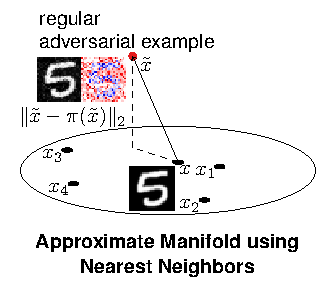
\includegraphics[width=1.05\textwidth]{fig/results_a1}
            \end{minipage}
            \begin{minipage}[t]{0.49\textwidth}
                \strut\vspace*{-\baselineskip} % !
                
                \centering
                
                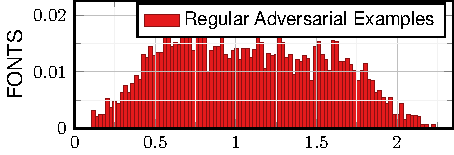
\includegraphics[width=1.05\textwidth]{fig/results_a2}
                
                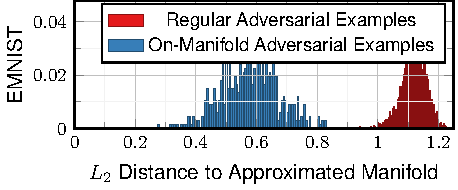
\includegraphics[width=1.05\textwidth]{fig/results_a3}
            \end{minipage}
            \vspace*{-1mm}
        \end{results}
        
        \vspace*{-1mm}
        \begin{results}{\Large\bf \fcolorbox{MPIIblue}{MPIIblue}{\hskip 0.05cm\color{MPIIwhite}4\hskip 0.05cm} Robustness Independent of Generalization}
            
            \centering
            \vspace*{-1.1mm}
            
            \hspace*{-2.5mm}
            \begin{minipage}[t]{0.32\textwidth}
                \strut\vspace*{-\baselineskip} % !
                
                \centering
                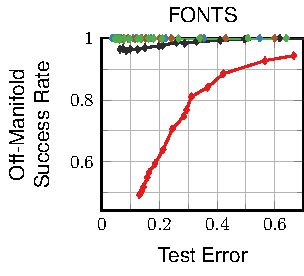
\includegraphics[width=1.05\textwidth]{fig/results_d1}
            \end{minipage}
            \hfill
            \begin{minipage}[t]{0.32\textwidth}
                \strut\vspace*{-\baselineskip} % !
                
                \centering
                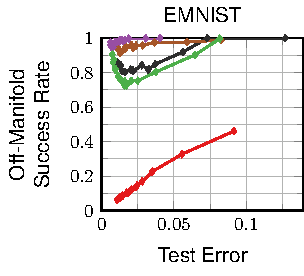
\includegraphics[width=1.05\textwidth]{fig/results_d2}
            \end{minipage}
            \hfill
            {\color{MPIIdarkgray}\unskip\vrule}
            \hfill
            \begin{minipage}[t]{0.29\textwidth}
                \strut\vspace*{-\baselineskip} % !
                
                \centering
                \vspace*{-0.5mm}
                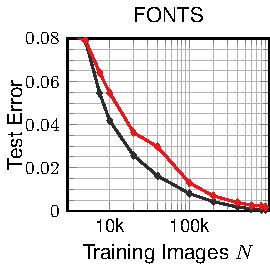
\includegraphics[width=1.05\textwidth]{fig/results_d3}
            \end{minipage}
        \end{results}
    
        \vspace*{-2.25mm}
        \begin{minipage}[t]{0.495\textwidth}
            \strut\vspace*{-\baselineskip} % !
            
            \begin{data}{\Large\bfseries FONTS (Synthetic)}
                \centering
                
                \vspace*{0.125mm}
                \hspace*{-0.6cm}
                \begin{tikzpicture}
                \begin{scope}[shift={(-0.5,0)},transform canvas={scale=0.75},overlay]
                \draw[thick,MPIIblack] (-1.5,1) rectangle (-1.25, 0.75);
                \draw[thick,MPIIblack] (-1.5,0.75) rectangle (-1.25, 0.5);
                \draw[thick,MPIIblack] (-1.5,0.5) rectangle (-1.25, 0.25);
                \draw[thick,MPIIblack] (-1.5,0.25) rectangle (-1.25, 0);
                \draw[thick,MPIIblack] (-1.5,0) rectangle (-1.25, -0.25);
                \draw[thick,MPIIblack] (-1.5,-0.25) rectangle (-1.25, -0.5);
                \draw[thick,MPIIblack] (-1.5,-0.5) rectangle (-1.25, -0.75);
                \draw[thick,MPIIblack] (-1.5,-0.75) rectangle (-1.25, -1);
                
                \draw[thick,MPIIblack] (-1.6,-1) -- (-1.75,-1) -- (-1.75,0.5) -- (-1.6,0.5);
                \draw[thick, MPIIblack] (-1.6,0.875) -- (-2, 0.875) -- (-2,1);
                \draw[thick, MPIIblack] (-1.6,0.625) -- (-2, 0.625);
                \end{scope}
                
                \node[anchor=south] at (-1.75, 0.7){\footnotesize character};
                \node[anchor=east] at (-1.75, 0.475){\footnotesize font};
                \node[anchor=east] at (-1.75, -0.25){\footnotesize \begin{tabular}{r@{}}affine\\tf\end{tabular}};
                
                \begin{scope}[shift={(-0.5,0)},transform canvas={scale=0.75},overlay]
                \draw[thick,MPIIblack] (-1,1) -- (1.5,2) -- (1.5,-2) -- (-1,-1) -- (-1,1);
                \end{scope}
                \node at (-0.15, 0){\footnotesize \begin{tabular}{c}deterministic\\decoder\end{tabular}};
                
                \node[anchor=west] at (0.75, 0){
\includegraphics[height=3cm,trim={16.5cm 12.5cm 0cm 0cm},clip]{gfx/fonts}};
                
                %\node at (0.5,-2){\large\bfseries Approximated Manifold};
                \end{tikzpicture}
            \end{data}
        \end{minipage}
        \hfill
        \begin{minipage}[t]{0.495\textwidth}
            \strut\vspace*{-\baselineskip} % !
            
            \begin{data}{\Large\bfseries EMNIST \vphantom{(Synthetic)}}
                \centering
                
                %\scalebox{0.65}{
                \begin{tikzpicture}
                \begin{scope}[shift={(3.35,-2.25)},transform canvas={scale=0.7}]
                \begin{scope} [shift={(-0.75,0)}]
                \node at (-5.7, 0){
\includegraphics[height=2cm]{gfx/experiments/emnist_learned_on_class/464_0_image_7.png}};
                \node[anchor=north] at (-5.7,-1){\Large \begin{tabular}{@{}c@{}}Image\end{tabular}};
                \draw[thick] (-4.6, 1) -- (-3.5, 0.35) -- (-3.5,-0.35) -- (-4.6,-1) -- (-4.6, 1);
                \node[] at (-4.1, 0){\Large \begin{tabular}{@{}c@{}}$\text{enc}$\end{tabular}};
                \end{scope}
                
                \node[rotate=90] at (-4, 0){
\includegraphics[height=0.175cm]{gfx/main/50_0_theta_original.png}};
                \node at (-3.3,0){\large ${+}0.16{\cdot}$};
                \node[rotate=90] at (-2.6, 0){
\includegraphics[height=0.175cm]{gfx/main/50_0_theta_perturbation.png}};
                \node[anchor=north] at (-3.3, -1){\Large \begin{tabular}{@{}c@{}}Perturbed\\ Latent Code\end{tabular}};
                
                \begin{scope}[shift={(-0.3,0)}]
                \draw[thick] (-1, 1) -- (-2.1, 0.35) -- (-2.1,-0.35) -- (-1,-1) -- (-1, 1);
                \node[] at (-1.5, 0){\Large \begin{tabular}{@{}c@{}}$\text{dec}$\end{tabular}};
                \node at (0.1, 0){
\includegraphics[height=2cm]{gfx/experiments/emnist_learned_on_class/464_1_attack_3.png}};
                \node[anchor=north] at (0.1, -1){\Large \begin{tabular}{@{}c@{}}Adversarial\\[-1px] Example\end{tabular}};
                %\draw[thick] (1.65, 1) -- (3.2, 0.35) -- (3.2,-0.35) -- (1.65,-1) -- (1.65, 1);
                %\node[] at (2.425, 0){\Large \begin{tabular}{@{}c@{}}$f(\tilde{x};w)$\end{tabular}};
                %\node[] at (3.5, 0){``3''};
                \end{scope}
                
                \draw[thick] (-6.5,1.1) -- (-6.5,1.75) -- (-4,1.75);
                \draw[thick] (-2.5,1.75) -- (-0.2, 1.75) -- (-0.2,1.1);
                \node at (-3.4, 1.75) {
\includegraphics[height=1.5cm]{{gfx/experiments/emnist_learned_on_class/464_1_perturbation_0.992153}.png}};
                %\node[anchor=south] at (-3.4, 2.35){\Large \begin{tabular}{@{}c@{}}Image Perturbation\end{tabular}};
                \end{scope}
                
                %\node at (-0,-2.5){\large\bfseries Approximated Manifold};
                \end{tikzpicture}
                %}
                \vspace*{32.45mm}
            \end{data}
        \end{minipage}
    \end{minipage}
    \hfill
    \begin{minipage}[t]{0.34\textwidth}
        \strut\vspace*{-\baselineskip} % !
        
        \begin{problem}{\Large\bfseries Problem}
            \large
            Investigating the relationship between \textbf{adversarial robustness} and \textbf{generalization} -- {\bfseries\color{MPIIblue} are accurate \emph{and} robust models possible?}
        \end{problem}
        
        \vspace*{-1mm}
        \begin{method}{\Large\bfseries Contributions}
            \begin{center}
                %set the plot display orientation
                %synatax: \tdplotsetdisplay{\theta_d}{\phi_d}
                \tdplotsetmaincoords{65}{20}
                %define xy plane
                \tikzset{yxplane/.style={canvas is yx plane at z=#1}}
                
                \scalebox{1.4}{
                \begin{tikzpicture}[scale=5,tdplot_main_coords,remember picture]
                
                \begin{scope}[yxplane=1]
                \draw[draw=black] (-0.5,0.85) -- (0.5, 0.85) arc(0:-180:0.5) -- cycle;
                \draw[white,thick](-0.5,0.85) -- (0.5,0.85);
                \fill[white,path fading=west] (-0.8,0.5) rectangle (0.6,0.9);
                
                
                \draw[thick,draw=MPIIblue] (-0.26,0.425) -- (0.26,0.425);
                \draw[thick,draw=MPIIred] (-0.3,0.4) -- (0.46,0.2);
                
                \draw[draw=black] (0,0) circle[radius=0.5cm] node{};
                
                \coordinate (o) at (0.1,0){};
                \draw[thick,draw=black,fill=black] (o) circle[radius=0.15mm] node{};
                %\node at ($(o) + (0.08,0.01)$){\footnotesize $x$};
                \end{scope}
                
                \coordinate (on1) at ($(o) + (0.275,0.2,0)$);
                %\node[anchor=north] at (on1){\footnotesize $\tilde{x}$};
                \draw[thick,draw=MPIIred,fill=MPIIred] (on1) circle[radius=0.1mm];
                \draw[->] (o) -- (on1);
                
                \coordinate (off) at ($(o) + (-0.2,0.1,0.25)$);
                %\node[anchor=south] at (off){\footnotesize $\tilde{x}$};
                \draw[thick,draw=MPIIred,fill=MPIIred] (off) circle[radius=0.1mm];
                \draw[->] (o) -- (off);
                \draw[-,dashed] (o) -- ($(o) + (-0.2,0.1,0)$);
                \draw[-,dashed] ($(o) + (-0.2,0.1,0)$) -- (off);
                
                \node[anchor=north east,yshift=0.1cm,xshift=0.05] at (off){
\includegraphics[width=0.75cm]{gfx/introduction/off_manifold/152_0_attack_9.png}
\includegraphics[width=0.75cm]{{gfx/introduction/off_manifold/152_0_perturbation_0.3}.png}};
                \node[anchor=south west,yshift=-0.1cm,xshift=-2.4cm] (c1) at (off){\small\bfseries \fcolorbox{MPIIblue}{MPIIblue}{\hskip 0.025cm\color{MPIIwhite}1\hskip 0.025cm}\color{MPIIblue}\hskip 0.1cm \begin{tabular}{@{}l@{}} regular\\[-1px] adversarial example\end{tabular}};
                
                \node[anchor=north east,xshift=0.05cm,yshift=0.05cm] at (o){
\includegraphics[width=0.75cm]{gfx/introduction/off_manifold/152_0_image_5.png}};
                
                \node[anchor=south west,xshift=-0.05cm,yshift=-0.05cm] at (on1){
\includegraphics[width=0.75cm]{gfx/introduction/on_manifold/152_0_attack_5}
\includegraphics[width=0.75cm]{{gfx/introduction/on_manifold/152_0_perturbation_0.901539}.png}};
                \node[anchor=south west,yshift=0.75cm,xshift=-0.725cm] (c2) at (on1){\small\bfseries \fcolorbox{MPIIblue}{MPIIblue}{\hskip 0.025cm\color{MPIIwhite}2\hskip 0.025cm}\color{MPIIblue}\hskip 0.1cm \begin{tabular}{@{}l@{}}on-manifold\\[-1px] adversarial example\end{tabular}};
                
                \node at ($(o) + (0.1,-0.7)$){\footnotesize Class Manifold ``5''};
                \node at ($(o) + (0.9,-0.7)$){\footnotesize Class Manifold ``6''};
                
                \node[anchor=west,MPIIblue,yshift=0.3cm] at (0.55,-0.3,1){\footnotesize \begin{tabular}{@{}c@{}}True\\Decision\\Boundary\end{tabular}};
                
                \node[anchor=north east,MPIIred,yshift=0.2cm] at (0.6,-0.4,1){\footnotesize \begin{tabular}{@{}c@{}}Classifier's\\Decision\\Boundary\end{tabular}};
                \end{tikzpicture}
                }
            \end{center}
            
            \large
            \color{MPIIblue}
            {\bfseries\fcolorbox{MPIIblue}{MPIIblue}{\hskip 0.05cm\color{MPIIwhite}\large 3\hskip 0.05cm} On-manifold robustness \emph{is} generalization.}
            \vskip 3px
            
            {\bfseries\fcolorbox{MPIIblue}{MPIIblue}{\hskip 0.05cm\color{MPIIwhite}\large 4\hskip 0.05cm} Regular robustness and generalization \emph{not} contradicting.\\[3px]
            \hspace*{6px}$\blacktriangleright$ Robustness has higher sample complexity.}
        \end{method}
    
        \vspace*{-2.5mm}
        \begin{minipage}[t]{0.85\textwidth}
            \strut\vspace*{-\baselineskip} % !
            
            \begin{code}{}\Large
                Paper, Code and Data:\\
                \bf\url{davidstutz.de/cvpr2019}
            \end{code}
        \end{minipage}
        \hfill
        \begin{minipage}[t]{0.14\textwidth}
            \strut\vspace*{-\baselineskip} % !
            
            \vspace*{-1.5mm}
            \hspace*{-2mm}
\includegraphics[width=23mm]{gfx/cvpr2019}
        \end{minipage}
    
        \vspace*{-2.5mm}
        \begin{moreresults}{}
            \vspace*{-0.75mm}
            \scalebox{0}{
    
\begin{tikzpicture}
    \begin{axis}[hide axis]
        \addplot [Normal,forget plot] coordinates{(1,1)};\label{plot:Normal}
        \addplot [OffAdvTrain,forget plot] coordinates{(1,1)};\label{plot:OffAdvTrain}
        \addplot [OnAdvTrain,forget plot] coordinates{(1,1)};\label{plot:OnAdvTrain}
        \addplot [OnClassAdvTrain,forget plot] coordinates{(1,1)};\label{plot:OnClassAdvTrain}
        \addplot [STNAdvTrain,forget plot] coordinates{(1,1)};\label{plot:STNAdvTrain}
        \addplot [STNAugm,forget plot] coordinates{(1,1)};\label{plot:STNAugm}
        \addplot [OnOffAdvTrain,forget plot] coordinates{(1,1)};\label{plot:OnOffAdvTrain}
        \addplot [OnOffClassAdvTrain,forget plot] coordinates{(1,1)};\label{plot:OnOffClassAdvTrain}
        \addplot [STNOffAdvTrain,forget plot] coordinates{(1,1)};\label{plot:STNOffAdvTrain}
        %
        \addplot [OffAdvTrain2,forget plot] coordinates{(1,1)};\label{plot:OffAdvTrain2}
        \addplot [OnAdvTrain2,forget plot] coordinates{(1,1)};\label{plot:OnAdvTrain2}
        \addplot [OnClassAdvTrain2,forget plot] coordinates{(1,1)};\label{plot:OnClassAdvTrain2}
        %
        \addplot [OffAdvTrain3,forget plot] coordinates{(1,1)};\label{plot:OffAdvTrain3}
        \addplot [OnAdvTrain3,forget plot] coordinates{(1,1)};\label{plot:OnAdvTrain3}
        \addplot [OnClassAdvTrain3,forget plot] coordinates{(1,1)};\label{plot:OnClassAdvTrain3}
        %
        \addplot [OffAugm,forget plot] coordinates{(1,1)};\label{plot:OffAugm}
        \addplot [OnAugm,forget plot] coordinates{(1,1)};\label{plot:OnAugm}
        \addplot [OnClassAugm,forget plot] coordinates{(1,1)};\label{plot:OnClassAugm}
        %
        \addplot [OnDataAdvTrain,forget plot] coordinates{(1,1)};\label{plot:OnDataAdvTrain}
        %
        \addplot[only marks,Normal,mark=triangle*,mark size=3pt,forget plot] coordinates{(1,1)};\label{plot:NormalScatter}
        \addplot[only marks,OffAdvTrain,mark=triangle*,mark size=3pt,forget plot] coordinates{(1,1)};\label{plot:OffAdvTrainScatter}
        \addplot[only marks,OnAdvTrain,mark=triangle*,mark size=3pt,forget plot] coordinates{(1,1)};\label{plot:OnAdvTrainScatter}
        \addplot[only marks,OnClassAdvTrain,mark=triangle*,mark size=3pt,forget plot] coordinates{(1,1)};\label{plot:OnClassAdvTrainScatter}
        \addplot[only marks,STNAdvTrain,mark=triangle*,mark size=3pt,forget plot] coordinates{(1,1)};\label{plot:STNAdvTrainScatter}
        \addplot[only marks,STNAugm,mark=triangle*,mark size=3pt,forget plot] coordinates{(1,1)};\label{plot:STNAugmScatter}
    \end{axis}
    \end{tikzpicture}
}
            
            \small
            \ref{plot:Normal} Normal Training\hspace*{0.15cm}
            \ref{plot:OffAdvTrain} Adversarial Training\\
            \ref{plot:OnAdvTrain} Adversarial Training with On-\emph{True}-Manifold Adversarial Examples\\
            \ref{plot:OnClassAdvTrain} Adversarial Training with On-\emph{Learned}-Manifold Adversarial Examples\\
            \ref{plot:STNAdvTrain} Adversarial Training with Adversarial Transformations
            
            \vspace*{-0.5mm}
            %\vspace*{1.3mm}
        \end{moreresults}
    \end{minipage}
    \hfill
    \begin{minipage}[t]{0.32\textwidth}
        \strut\vspace*{-\baselineskip} % !
        
        \begin{results}{\Large\bf \fcolorbox{MPIIblue}{MPIIblue}{\hskip 0.05cm\color{MPIIwhite}2\hskip 0.05cm} On-Manifold Adversarial Examples}
            \vspace*{-2mm}
            
            \centering
            \hspace*{-3mm}
            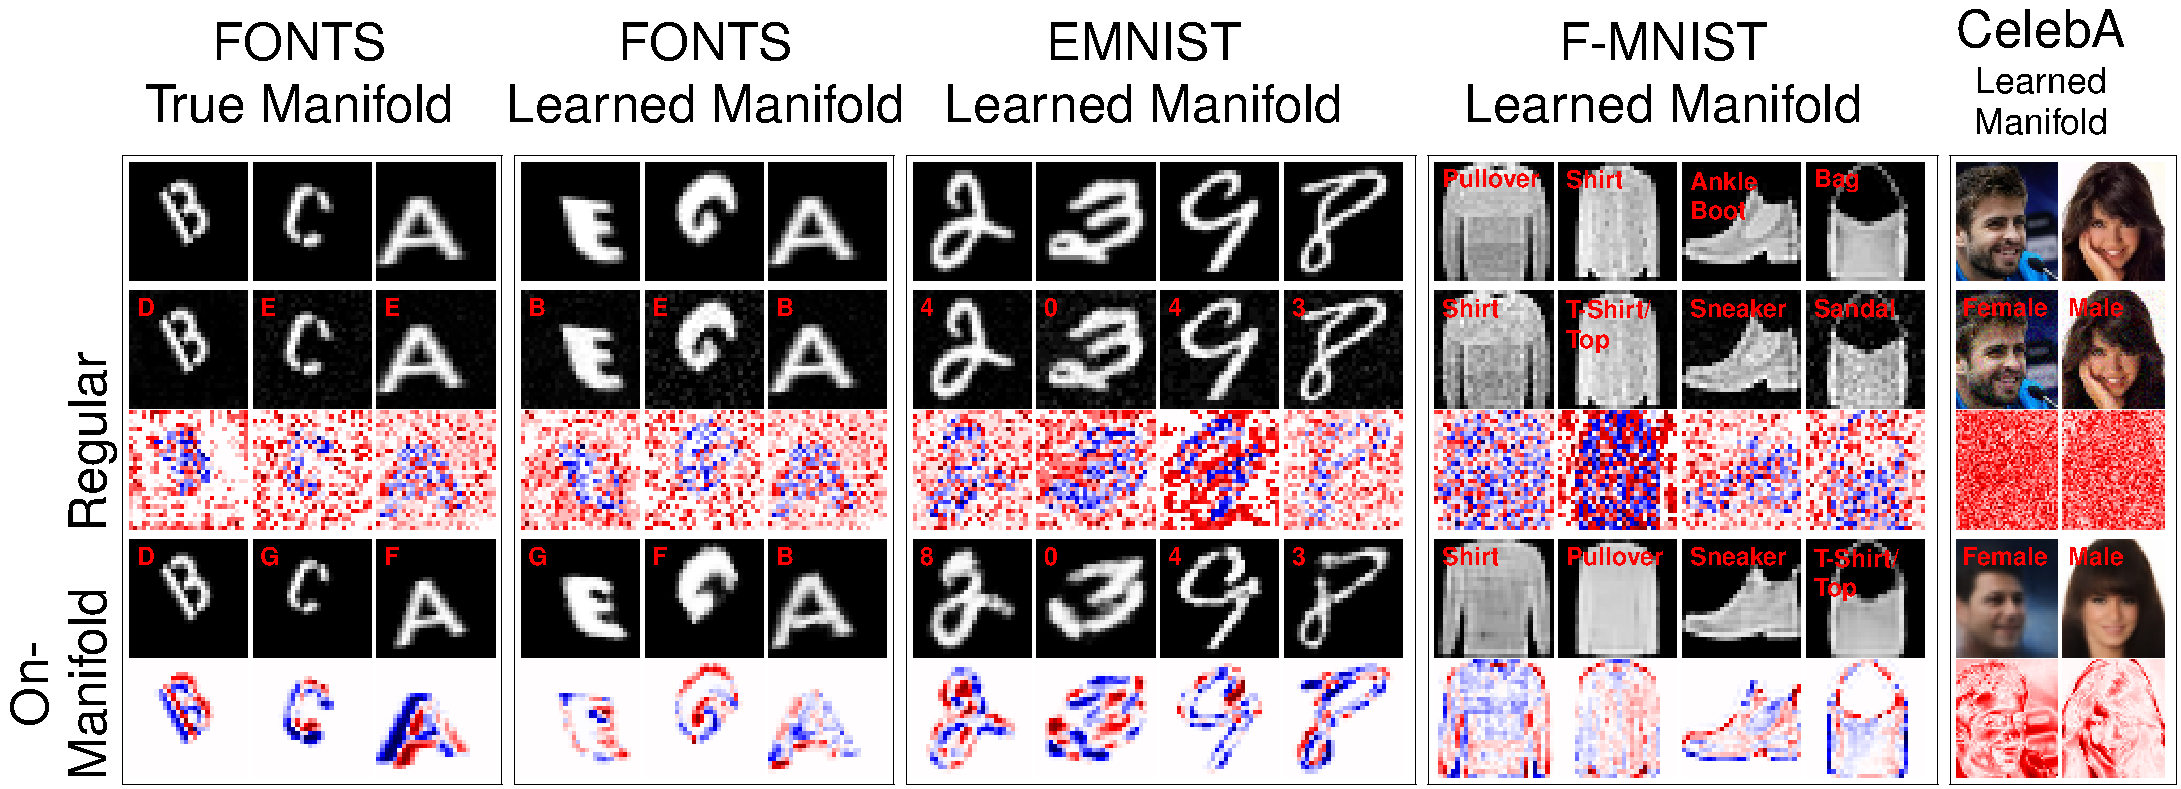
\includegraphics[width=1.03\textwidth]{fig/results_b4}
        \end{results}
        
        \vspace*{-1mm}
        \begin{results}{\Large\bf \fcolorbox{MPIIblue}{MPIIblue}{\hskip 0.05cm\color{MPIIwhite}3\hskip 0.05cm} On-Manifold Robustness \emph{is} Generalization}
            
            \centering
            
           	\large 
           	\vspace*{-1mm}
               
            \hspace*{-2.5mm}
           	\begin{minipage}[t]{0.3\textwidth}
           		\strut\vspace*{-\baselineskip} % !
           		
           		\centering
           		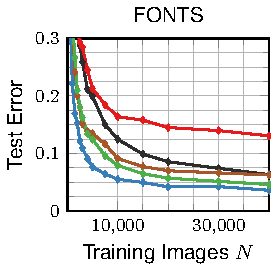
\includegraphics[width=1.05\textwidth]{fig/results_c5}
       		\end{minipage}
            \hfill
           	\begin{minipage}[t]{0.3\textwidth}
           		\strut\vspace*{-\baselineskip} % !
           		
           		\centering
           		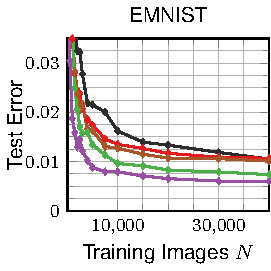
\includegraphics[width=1.05\textwidth]{fig/results_c6}
           	\end{minipage}
            \hfill
            {\color{MPIIdarkgray}\unskip\vrule}
            \hfill
            \begin{minipage}[t]{0.34\textwidth}
                \strut\vspace*{-\baselineskip} % !
                
                \centering
                \vspace*{-0.5mm}
                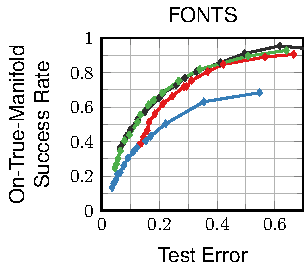
\includegraphics[width=1.05\textwidth]{fig/results_c2}
            \end{minipage}
        \end{results}
    
        \vspace*{-1mm}
        \begin{related}{\Large\bfseries Related Work}
            \large
            \begin{itemize}
                \item \cite{TsiprasARXIV2018,SuARXV2018}: trade-off between robustness and generalization;
                \item \cite{TanayARXIV2016,GilmerARXIV2018}: off- or on-manifold adversarial examples.
            \end{itemize}
        \end{related}
    
        \vspace*{-1mm}
        \begin{references}{}
            \vspace*{-0.05mm}
            \AtNextBibliography{\fontsize{7}{9}\selectfont}
            {\begingroup
                \color{MPIIdarkergray}
                %\fontsize{2.5}{4}\selectfont
                \renewcommand{\section}[2]{}%
                \printbibliography
                \endgroup}
            \vspace*{-0.45mm}
        \end{references}
    \end{minipage}
    \begin{tikzpicture}[overlay,remember picture]
        %\draw[-,line width=0.5mm,draw=MPIIblue] ($(c1) + (-1.75,1.5)$) -- (cc1);
        %\draw[-,line width=0.5mm,draw=MPIIblue] ($(c2) + (3.25 ,1.5)$) -- (cc2);
        %\draw[-,line width=0.5mm,draw=MPIIblue] ($(c3) + (3.25,1.5)$) -- (cc3);
        %\draw[-,line width=0.5mm,draw=MPIIblue] ($(c4) + (3.25,1.5)$) -- (cc4);
    \end{tikzpicture}
\end{document}
